\subsection{Design of the Motor Loop Controller}\label{sec:MotorLoop}

The very first loop control is the one adjusting the motor velocity, $\omega_m$, according to the voltage. The transfer function from $U_m$ to $\omega_{m}$ is taken from \autoref{sec:ModelDCMotor}. The values for the variables in \autoref{eq:DCModelNoL} is inserted giving \autoref{eq:MotorWithValues}.
\begin{flalign}\label{eq:MotorWithValues}
\frac{\Omega_m(s)}{U_m(s)}=\frac{201.24}{s+14.11} 
\end{flalign} 

As it is the most inner loop of the system, the step response has to be faster than the outer loops controlling the arm and the stick. The transfer function has a negative pole making the system stable. It also has a pretty large gain already so simply closing the loop is enough to get a faster response. The step response of the closed motor loop is seen on \autoref{fig:MotorStepClosed}.
\begin{figure}[htbp]
\centering
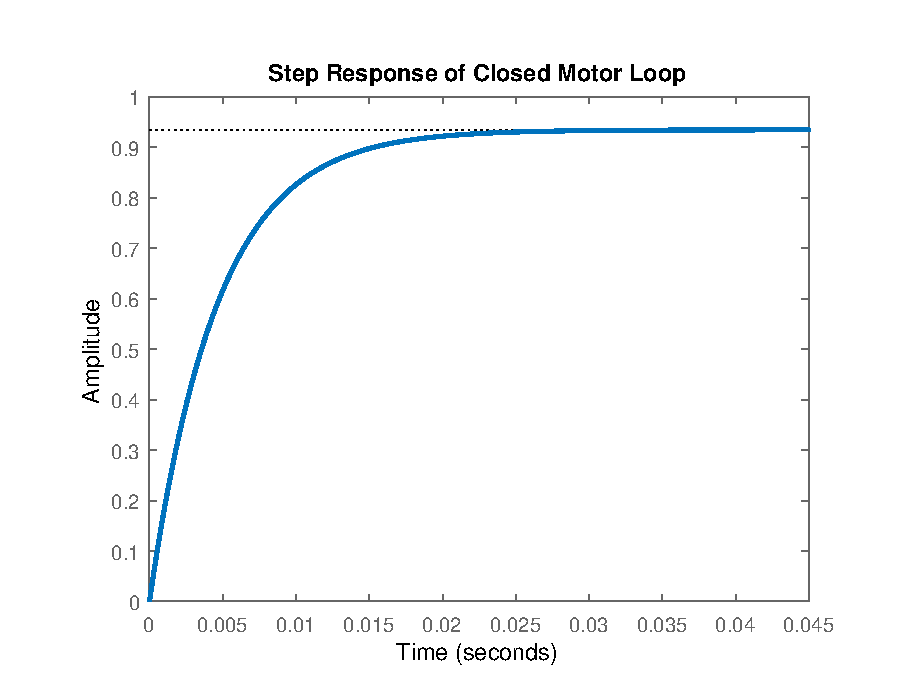
\includegraphics[width=0.7\textwidth]{MotorStepClosed}
\caption{Step response of the closed motor loop with a gain of 1.}
\label{fig:MotorStepClosed}
\end{figure}

There is a small steady state error that will be corrected slightly by increasing the gain. The gain is increased until the steady state error is less than 5\%. The gain required is 1.35. The step response of the closed motor loop with a gain of 1.35 can be seen on \autoref{fig:MotorStepGain}. This has a settling time of 0.0137 seconds.

\begin{figure}[htbp]
\centering
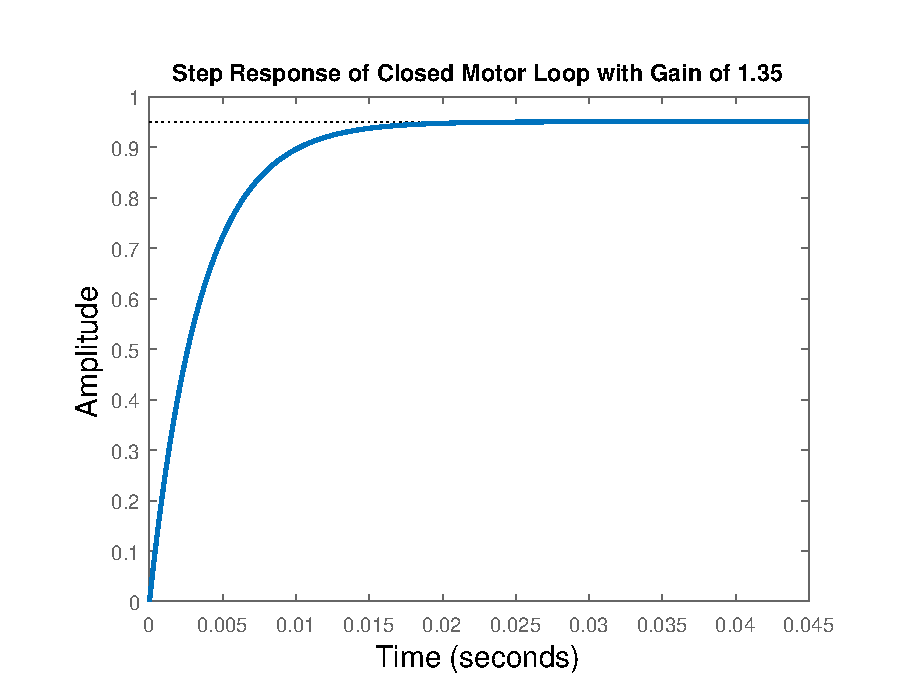
\includegraphics[width=0.7\textwidth]{MotorStepGain}
\caption{Step response of the closed motor loop with a gain of 1.35.}
\label{fig:MotorStepGain}
\end{figure}
\newpage

The controller for the motor loop thus becomes \autoref{eq:MotorController}.
\begin{flalign}\label{eq:MotorController}
D_{motor}=1.35
\end{flalign}

%The root locus of the motor loop is seen on \autoref{fig:MotorRootLocus}.
%\begin{figure}[htbp]
%\centering
%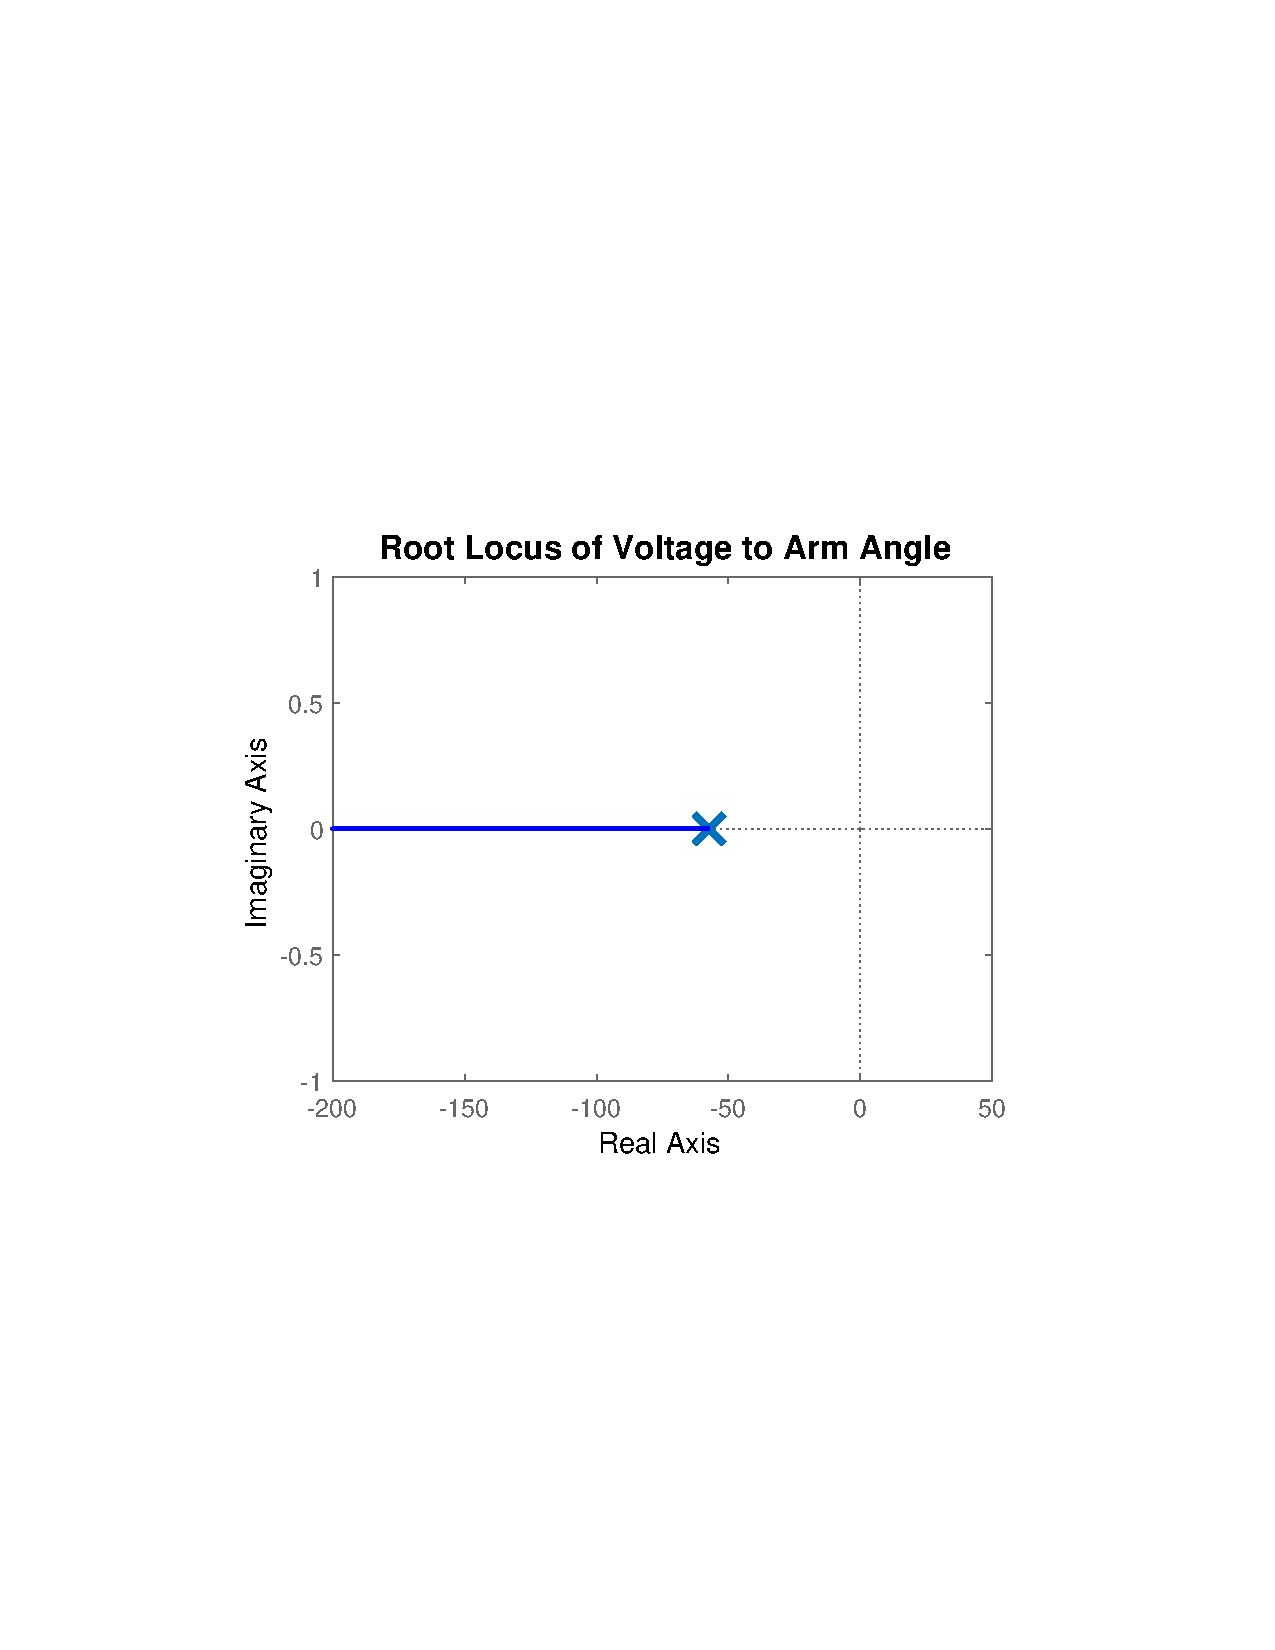
\includegraphics[width=\textwidth]{figures/Design/MotorLoop/MotorRootLocus}
%\caption{Root locus of the motor transfer function.}
%\label{fig:MotorRootLocus}
%\end{figure}


%\end{subfigure}
%\begin{subfigure}{0.48\textwidth}
%\centering
%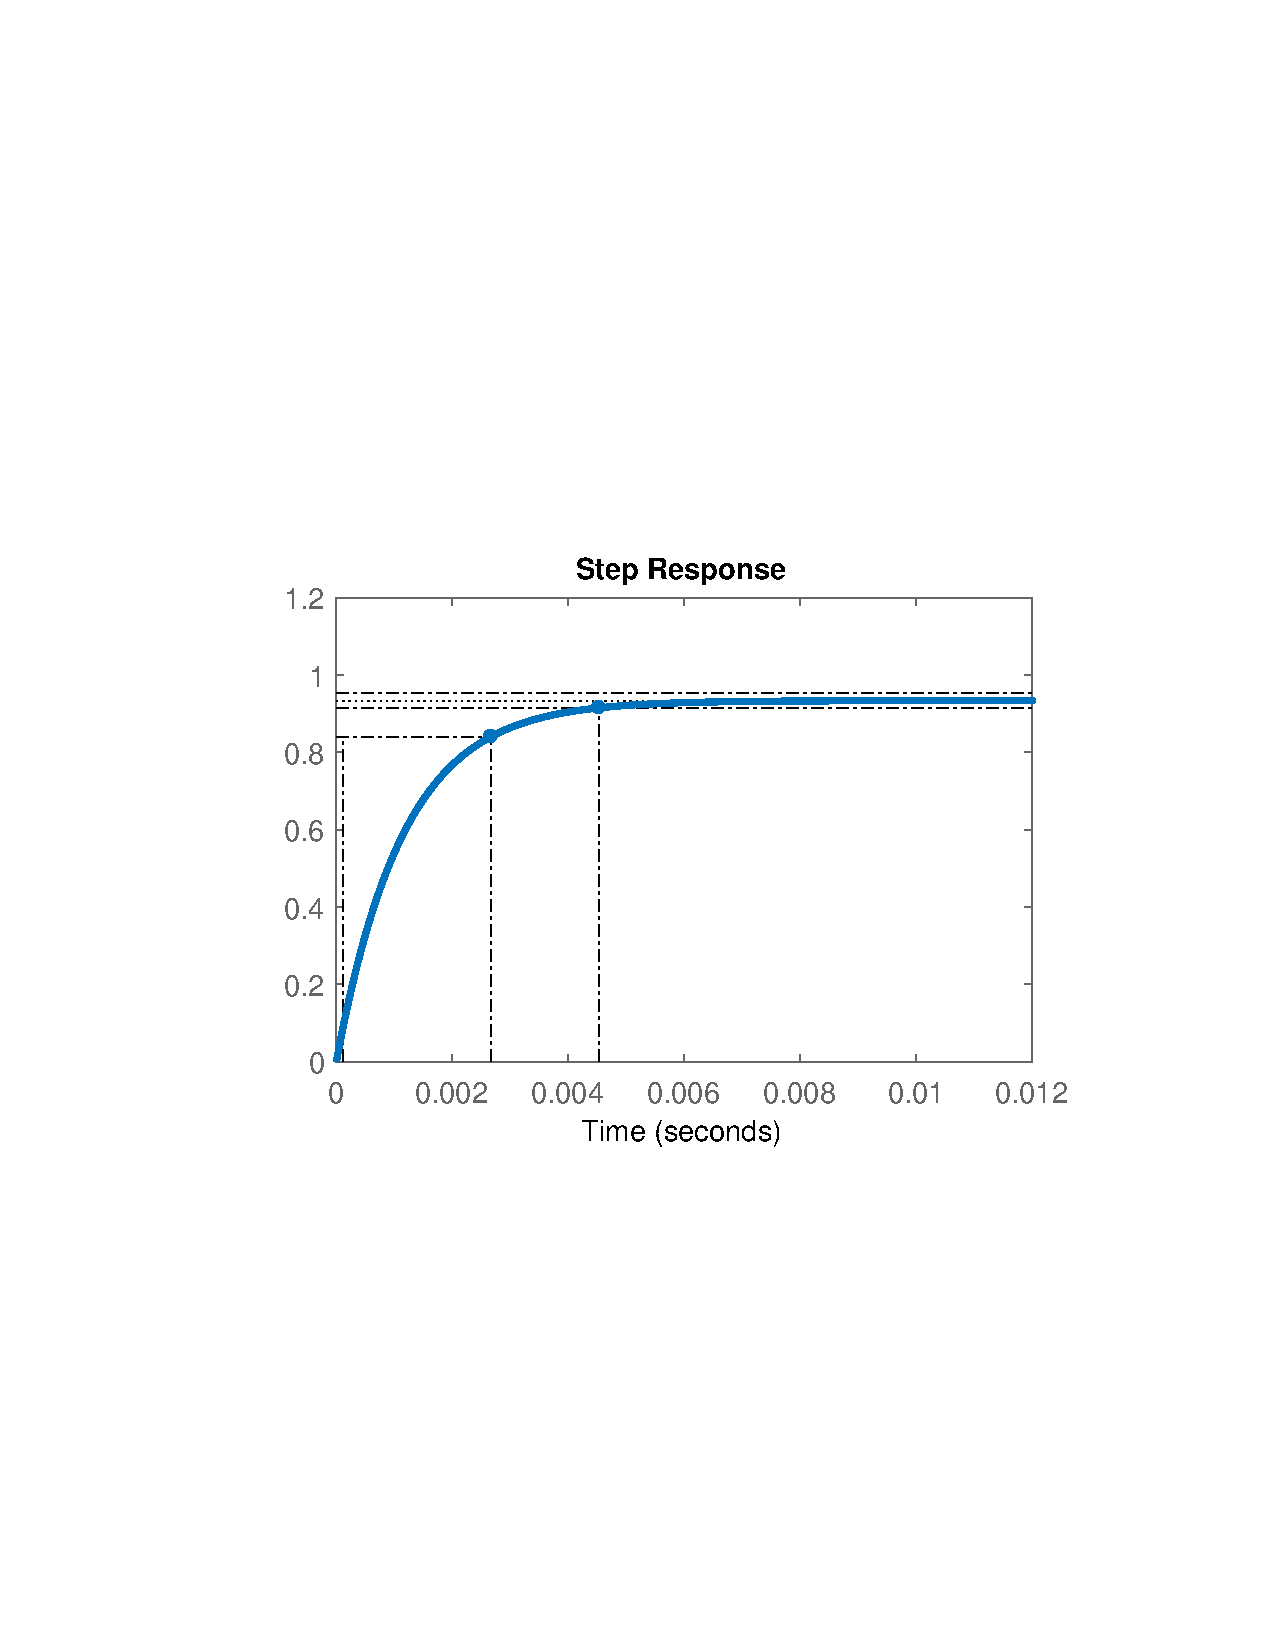
\includegraphics[width=\textwidth]{figures/Design/MotorLoop/MotorStepUncontrolled}
%\caption{Step response of the uncontrolled close loop transfer function.}
%\label{fig:MotorStepUncontrolled}
%\end{subfigure}
%\caption{Root locus and step response of the motor loop.}
%\label{fig:MotorRlocusStep}

%\autoref{fig:MotorRootLocus} confirms that the motor loop is naturally stable. However, there is a steady state error. The gain is increased until the steady state error is negligible. A proportional gain of 7 is sufficient. 
%
%As seen on \autoref{fig:MotorStepControlled}, the controlled loop has a rise time of 0.27 ms, ten times faster than the uncontrolled loop. Moreover, the steady state error has decreased from 7\% to 0.01\%. With a proportional gain of 10, the pole is moved far in the left half plane making the motor loop fast enough to be considered as a wire for the arm.
%\begin{figure}[htbp]
%	\centering
%	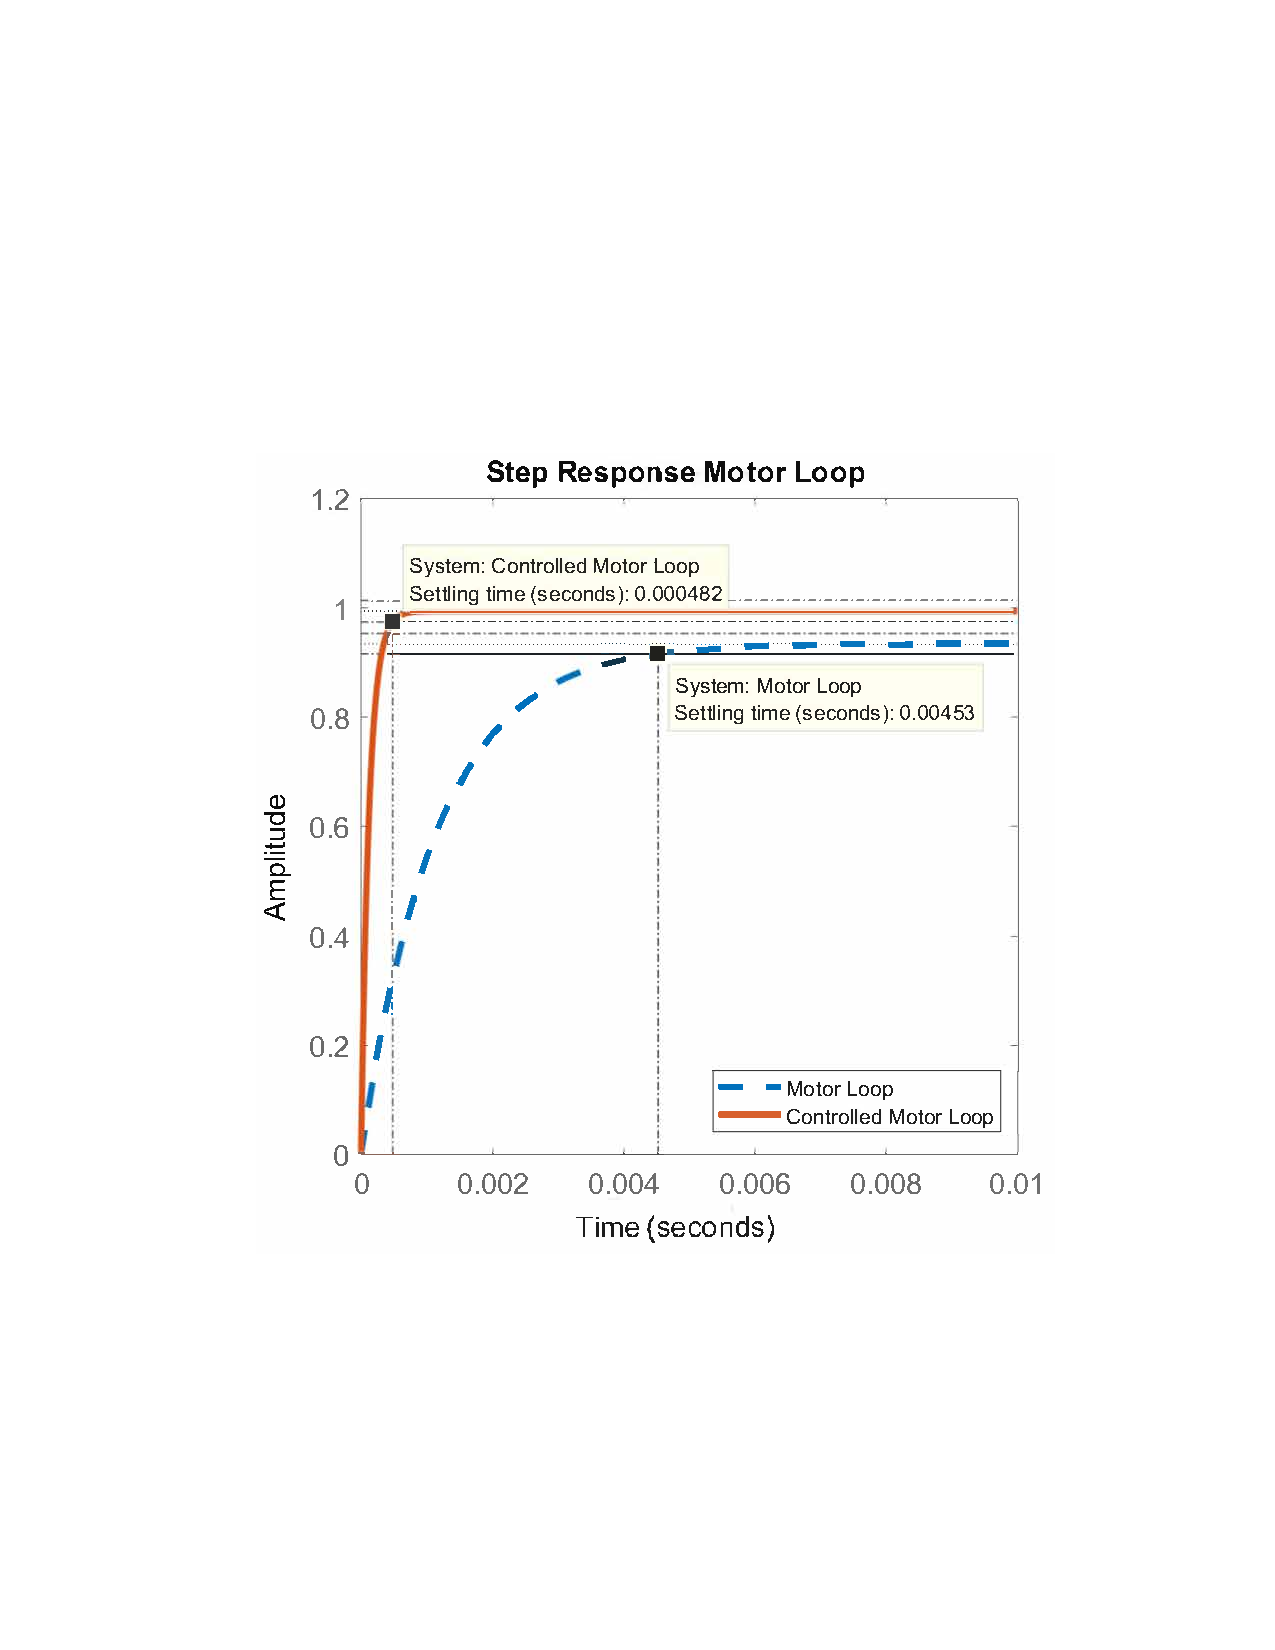
\includegraphics[width=0.7\textwidth]{figures/Design/MotorLoop/MotorStepControlled}
%	\caption{Step response of the controlled motor loop.}
%	\label{fig:MotorStepControlled}
%\end{figure}
